
\section{Introduction}

  O Flappy Bird is a game developed by Vietnamese programmer Dong Nguyen. The game, the player controls a bird, attempting to fly between columns of green pipes without hitting them. 
  The game was released in May 2013 but received a sudden rise in popularity in early 2014 and became a sleeper hit. Flappy Bird received poor reviews from some critics, who criticized its high level of difficulty and alleged plagiarism in graphics and game mechanics, while other reviewers found it addictive. 
  Flappy Bird was removed from both the App Store and Google Play by its creator on February 10, 2014. He claims that he felt guilt over what he considered to be its addictive nature and overuse.

  \begin{figure}[H]
  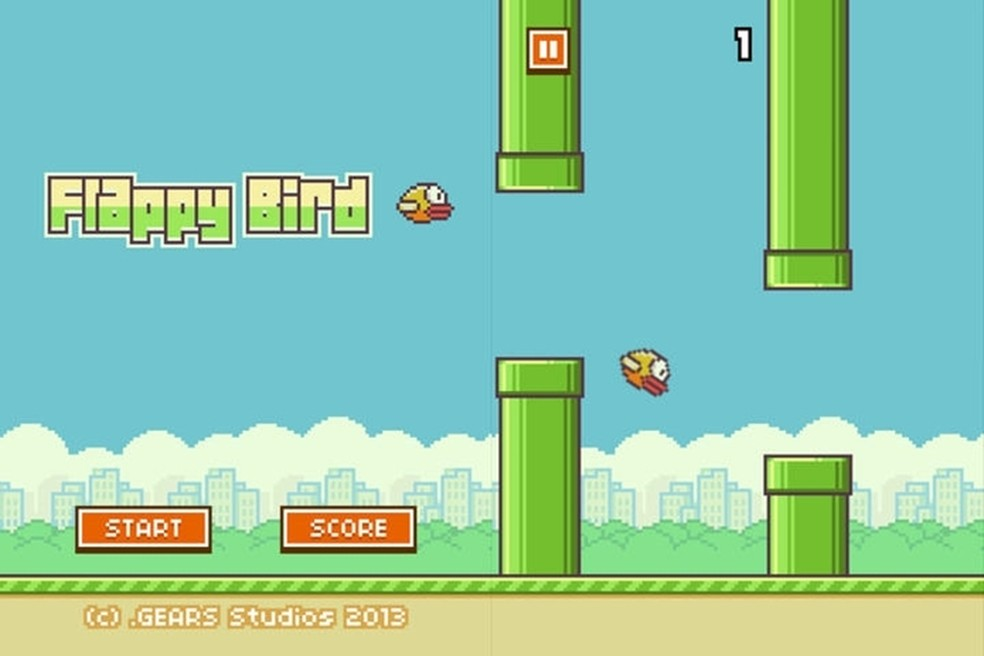
\includegraphics[width=8cm, height=5cm]{figuras/flappy-bird.jpeg}
  \caption{Flappy Bird Game}
  \end{figure} 
  
 
  The Reinforcement learning techniques will be implemented using the OpenIA Gym toolkit. OpenIA Gym has an open source interface for reinforcement learning tasks.
  The academy library offers an easy-to-use set of remedial learning tasks.
  Briefly, OpenIA Gym is a python library that gives us a large number of test environments to work on algorithms with shared interfaces
  
  \begin{figure}[H]
  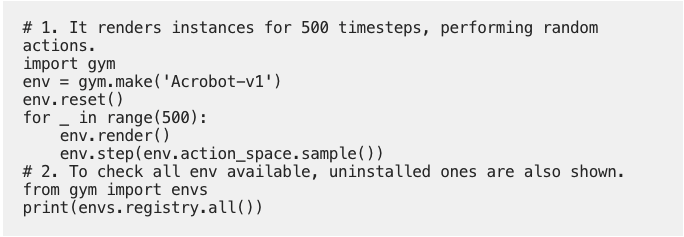
\includegraphics[width=8cm, height=4cm]{figuras/openIA_code_example.png}
  \caption{Flappy Bird Game}
  \end{figure} 
